\documentclass{prova}

\usepackage{amssymb}
\usepackage{gensymb}

\renewcommand{\sin}{\mbox{sen}}
\newcommand{\ra}{\rightarrow}
\newcommand{\lra}{\leftrightarrow}
\newcommand{\Ra}{\Rightarrow}
\newcommand{\LRa}{\Leftrightarrow}
\renewcommand{\lnot}{\sim}
\newcommand{\larg}{\vdash}
\newcommand{\ds}{\displaystyle}
\newcommand{\sen}{\mathop\mathrm{sen}\nolimits}
\newcommand{\tg}{\mathop\mathrm{tg}\nolimits}

\professor{Prof. Adriano Barbosa}
\disciplina{Introdução ao Cálculo}
\avaliacao{Final}
\curso{Matem\'atica}
\data{17/12/2020}

\begin{document}
    \cabecalho{5}  % o numero 5 indica a qnt de quadros na tabela de nota
    
    \textbf{Todas as respostas devem ser justificadas.}
    \begin{questionario}
        \q{A velocidade instantânea no tempo $t$ de um corpo que se move
           segundo uma função $s(t)$, onde $s(t)$ descreve o deslocamento do corpo em
           função do tempo, é dada por:
           \[v(t) = \lim_{h\rightarrow t} \ds\frac{s(h)-s(t)}{h-t}.\]}
           \begin{questionario}
               \qq{Encontre a função que descreve a velocidade instantânea de
                   um corpo que se move segundo a função $s(t)=t^2+t$.}
               \qq{Determine a velocidade instântanea em $t=1$.}
           \end{questionario}
        \q{Dados os intervalos da forma $\ds\left[0, \frac{1}{n}\right]$, com
           $n\in\mathbb{N}$. Pergunta-se:}
            \begin{questionario}
                \qq{Existe algum número real comum a todos os intervalos?}
                \qq{E se os intervalos fossem abertos,
                    $\ds\left(0,\frac{1}{n}\right)$, com $n\in\mathbb{N}$?}
            \end{questionario}
        \q{Uma sequência com 2020 hexágonos foi montada como na figura abaixo.
           Quantas arestas existem na sequência?}
           \begin{figure}[h]
               \centering
               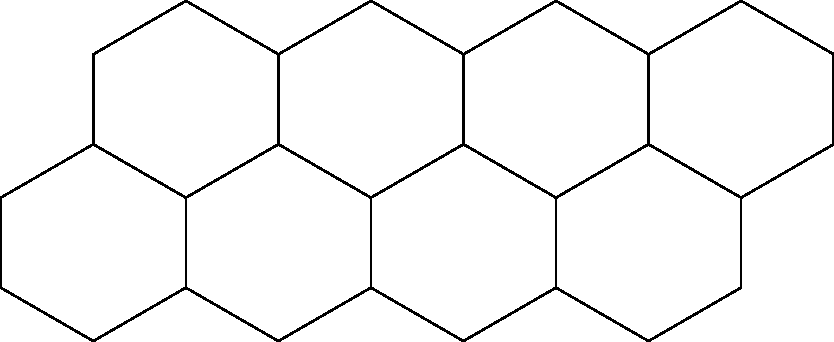
\includegraphics[width=0.5\textwidth]{fig1.pdf}
           \end{figure}
        \q{Calcule $\sen{x}$ e $\cos{x}$ sabendo que $\tg{x}+\sec{x}=\ds\frac{3}{2}$.}
        \pagebreak{}
        \q{Escreva cada uma das funções quadráticas abaixo na forma
           $f(x)=a(x-m)^2+k$. A seguir, calcule suas raízes (se existirem), o eixo de
           simetria de seu gráfico, seus valores máximo e mínimo e os valores de $x$ onde
           ocorrem.}
            \begin{questionario}
                \qq{$f(x)=2x^2-16x+29$}
                \qq{$f(x)=-x^2+\ds\frac{2}{3}x+\frac{17}{9}$}
            \end{questionario}
        \q{Sejam
           \[f:\mathbb{R}\rightarrow\mathbb{R}, f(x)=\ds\frac{1}{5}\ 2^x\]
           \[g:\mathbb{R}^{+}\rightarrow\mathbb{R}, g(x)=\log_{10} x.\]
           Esboce o gráfico da composta $g(f(x))$ sem utilizar softwares ou
           calculadoras gráficas. Justifique os passos.}
    \end{questionario}
\end{document}
